% Options for packages loaded elsewhere
\PassOptionsToPackage{unicode}{hyperref}
\PassOptionsToPackage{hyphens}{url}
%
\documentclass[
  letterpaper,
]{book}

\usepackage{amsmath,amssymb}
\usepackage{iftex}
\ifPDFTeX
  \usepackage[T1]{fontenc}
  \usepackage[utf8]{inputenc}
  \usepackage{textcomp} % provide euro and other symbols
\else % if luatex or xetex
  \usepackage{unicode-math}
  \defaultfontfeatures{Scale=MatchLowercase}
  \defaultfontfeatures[\rmfamily]{Ligatures=TeX,Scale=1}
\fi
\usepackage{lmodern}
\ifPDFTeX\else  
    % xetex/luatex font selection
\fi
% Use upquote if available, for straight quotes in verbatim environments
\IfFileExists{upquote.sty}{\usepackage{upquote}}{}
\IfFileExists{microtype.sty}{% use microtype if available
  \usepackage[]{microtype}
  \UseMicrotypeSet[protrusion]{basicmath} % disable protrusion for tt fonts
}{}
\makeatletter
\@ifundefined{KOMAClassName}{% if non-KOMA class
  \IfFileExists{parskip.sty}{%
    \usepackage{parskip}
  }{% else
    \setlength{\parindent}{0pt}
    \setlength{\parskip}{6pt plus 2pt minus 1pt}}
}{% if KOMA class
  \KOMAoptions{parskip=half}}
\makeatother
\usepackage{xcolor}
\usepackage[twoside]{geometry}
\setlength{\emergencystretch}{3em} % prevent overfull lines
\setcounter{secnumdepth}{5}
% Make \paragraph and \subparagraph free-standing
\ifx\paragraph\undefined\else
  \let\oldparagraph\paragraph
  \renewcommand{\paragraph}[1]{\oldparagraph{#1}\mbox{}}
\fi
\ifx\subparagraph\undefined\else
  \let\oldsubparagraph\subparagraph
  \renewcommand{\subparagraph}[1]{\oldsubparagraph{#1}\mbox{}}
\fi


\providecommand{\tightlist}{%
  \setlength{\itemsep}{0pt}\setlength{\parskip}{0pt}}\usepackage{longtable,booktabs,array}
\usepackage{calc} % for calculating minipage widths
% Correct order of tables after \paragraph or \subparagraph
\usepackage{etoolbox}
\makeatletter
\patchcmd\longtable{\par}{\if@noskipsec\mbox{}\fi\par}{}{}
\makeatother
% Allow footnotes in longtable head/foot
\IfFileExists{footnotehyper.sty}{\usepackage{footnotehyper}}{\usepackage{footnote}}
\makesavenoteenv{longtable}
\usepackage{graphicx}
\makeatletter
\def\maxwidth{\ifdim\Gin@nat@width>\linewidth\linewidth\else\Gin@nat@width\fi}
\def\maxheight{\ifdim\Gin@nat@height>\textheight\textheight\else\Gin@nat@height\fi}
\makeatother
% Scale images if necessary, so that they will not overflow the page
% margins by default, and it is still possible to overwrite the defaults
% using explicit options in \includegraphics[width, height, ...]{}
\setkeys{Gin}{width=\maxwidth,height=\maxheight,keepaspectratio}
% Set default figure placement to htbp
\makeatletter
\def\fps@figure{htbp}
\makeatother
% definitions for citeproc citations
\NewDocumentCommand\citeproctext{}{}
\NewDocumentCommand\citeproc{mm}{%
  \begingroup\def\citeproctext{#2}\cite{#1}\endgroup}
\makeatletter
 % allow citations to break across lines
 \let\@cite@ofmt\@firstofone
 % avoid brackets around text for \cite:
 \def\@biblabel#1{}
 \def\@cite#1#2{{#1\if@tempswa , #2\fi}}
\makeatother
\newlength{\cslhangindent}
\setlength{\cslhangindent}{1.5em}
\newlength{\csllabelwidth}
\setlength{\csllabelwidth}{3em}
\newenvironment{CSLReferences}[2] % #1 hanging-indent, #2 entry-spacing
 {\begin{list}{}{%
  \setlength{\itemindent}{0pt}
  \setlength{\leftmargin}{0pt}
  \setlength{\parsep}{0pt}
  % turn on hanging indent if param 1 is 1
  \ifodd #1
   \setlength{\leftmargin}{\cslhangindent}
   \setlength{\itemindent}{-1\cslhangindent}
  \fi
  % set entry spacing
  \setlength{\itemsep}{#2\baselineskip}}}
 {\end{list}}
\usepackage{calc}
\newcommand{\CSLBlock}[1]{\hfill\break\parbox[t]{\linewidth}{\strut\ignorespaces#1\strut}}
\newcommand{\CSLLeftMargin}[1]{\parbox[t]{\csllabelwidth}{\strut#1\strut}}
\newcommand{\CSLRightInline}[1]{\parbox[t]{\linewidth - \csllabelwidth}{\strut#1\strut}}
\newcommand{\CSLIndent}[1]{\hspace{\cslhangindent}#1}

\usepackage{amsthm}
\usepackage{lipsum}
\makeatletter
\@ifpackageloaded{bookmark}{}{\usepackage{bookmark}}
\makeatother
\makeatletter
\@ifpackageloaded{caption}{}{\usepackage{caption}}
\AtBeginDocument{%
\ifdefined\contentsname
  \renewcommand*\contentsname{Table of contents}
\else
  \newcommand\contentsname{Table of contents}
\fi
\ifdefined\listfigurename
  \renewcommand*\listfigurename{List of Figures}
\else
  \newcommand\listfigurename{List of Figures}
\fi
\ifdefined\listtablename
  \renewcommand*\listtablename{List of Tables}
\else
  \newcommand\listtablename{List of Tables}
\fi
\ifdefined\figurename
  \renewcommand*\figurename{Figure}
\else
  \newcommand\figurename{Figure}
\fi
\ifdefined\tablename
  \renewcommand*\tablename{Table}
\else
  \newcommand\tablename{Table}
\fi
}
\@ifpackageloaded{float}{}{\usepackage{float}}
\floatstyle{ruled}
\@ifundefined{c@chapter}{\newfloat{codelisting}{h}{lop}}{\newfloat{codelisting}{h}{lop}[chapter]}
\floatname{codelisting}{Listing}
\newcommand*\listoflistings{\listof{codelisting}{List of Listings}}
\makeatother
\makeatletter
\makeatother
\makeatletter
\@ifpackageloaded{caption}{}{\usepackage{caption}}
\@ifpackageloaded{subcaption}{}{\usepackage{subcaption}}
\makeatother
\ifLuaTeX
  \usepackage{selnolig}  % disable illegal ligatures
\fi
\usepackage{bookmark}

\IfFileExists{xurl.sty}{\usepackage{xurl}}{} % add URL line breaks if available
\urlstyle{same} % disable monospaced font for URLs
\hypersetup{
  pdftitle={Computational Approaches to Biofoundry-based Protein Engineering and Synthetic Biology},
  pdfauthor={Aporva Gupta},
  hidelinks,
  pdfcreator={LaTeX via pandoc}}

\title{Computational Approaches to Biofoundry-based Protein Engineering
and Synthetic Biology}
\author{Aporva Gupta}
\date{}

\begin{document}
\frontmatter
\maketitle

\renewcommand*\contentsname{Table of contents}
{
\setcounter{tocdepth}{2}
\tableofcontents
}
\mainmatter
\bookmarksetup{startatroot}

\chapter*{Abstract}\label{abstract}
\addcontentsline{toc}{chapter}{Abstract}

\markboth{Abstract}{Abstract}

\#TODO

\bookmarksetup{startatroot}

\chapter*{Introduction}\label{introduction}
\addcontentsline{toc}{chapter}{Introduction}

\markboth{Introduction}{Introduction}

\section*{Outline of Chapters}\label{outline-of-chapters}
\addcontentsline{toc}{section}{Outline of Chapters}

\markright{Outline of Chapters}

\bookmarksetup{startatroot}

\chapter{Computational Tools for Streamlined Biofoundry
Workflows}\label{computational-tools-for-streamlined-biofoundry-workflows}

\section{Introduction}\label{introduction-1}

The Design-Build-Test-Learn (DBTL) cycle, a foundational methodology of
synthetic biology, adopts engineering principles to enhance
reproducibility and efficiency in biological research. Yet, the Build
and Test phases pose considerable challenges to their labor-intensive
and time-consuming nature. For instance, the assembly of three DNA
fragments often requires a week per circuit assembly by a skilled
graduate student. Furthermore, optimizing the expression of a gene with
promoters, RBSs, and terminator parts - three different types for each
-- necessitates creating and testing 27 distinct DNA combinations. This
process could extend a graduate student's workload to four to six months
for the construction of an optimal genetic circuit.

On an industrial scale, the Build and Test stages present similarly
formidable challenges. The development and commercialization of
Artemisinin, a treatment for malaria by Amyris, demanded an investment
of \$15 million and ten years, equivalent to roughly 150 person-years.
Similarly, DuPont's production of 1,3-propanediol required 575
person-years, highlighting the extensive resource commitment in
synthetic biology projects {[}1{]}. These instances underline the
significant time and labor investments needed to harness the benefits of
synthetic biology, explaining why the field, which emerged in the early
2000s, took about a decade to prove its value.

The incorporation of robotics into biology has significantly reduced the
manual labor and time constraints traditionally associated with
biological experiments. This advancement was pioneered by Dr.~Ross D.
King in 2004 {[}2{]}, who developed the robotic scientists Adam and Eve
to autonomously investigate yeast metabolism and enzyme discovery
{[}3{]}. Despite their innovative potential, the application of these
robotic scientists has faced limitations due to the need for specialized
automation equipment tailored for specific research projects. This
requirement often limits the flexibility needed to conduct a wide array
of complex biological experiments, leading to significant costs and
efforts to adapt commercial equipment for various research needs.

However, the fundamental principles of synthetic biology, including
standardized parts, assembly techniques, and an engineering-focused DBTL
strategy, have demonstrated significant compatibility with automation
and robotics. This synergy has not only enhanced research but also found
practical industrial applications. A notable example is Lanzatech's
production of ethanol from greenhouse gases using its
clostridiaBiofoundry (cBioFab) {[}4{]}, which combines cell-free systems
with machine learning technology to achieve remarkable industrial
breakthroughs {[}5, 6{]} in producing 1-hexanol and hexanoic acid
(\textgreater100x improvement).

A biofoundry integrates the entire DBTL cycle, from initial DNA design
to testing cells modified with that DNA, by systematically linking
automated hardware and software to streamline the process from gene
synthesis to the final product. A key strategy in constructing an
efficient biofoundry is the careful design of each DBTL stage to ensure
seamless operation and eliminate bottlenecks, significantly improving
development speed and throughput. For instance, Ginkgo Bioworks has
shown considerable efficiency gains, with its throughput increasing two
to four times annually between 2014 and 2020. In 2017, the company
achieved a milestone when the cost of testing per strain became lower
than that of manual handling {[}7{]}. Amyris, having launched its
biofoundry in 2011, has successfully commercialized 15 new substances at
a consistent rate over the last seven years {[}8{]}, marking a
productivity increase of more than twentyfold compared to its earlier
efforts with Artemisinin. These developments underscore the
transformative impact of biofoundries on synthetic biology, providing
scalable and cost-efficient solutions for bioproduct development. By
optimizing the bioproduct development process, biofoundries
substantially reduce the time and cost associated with bringing new
products to market, representing a significant advancement in
biotechnological innovation.

\section{Considerations required for biofoundry
development}\label{considerations-required-for-biofoundry-development}

\subsection{Hardware}\label{hardware}

The concept of a biofoundry often evokes images of automated robotics
operating within a biological laboratory. Given this association,
automation is deemed essential for the development of biofoundries.
However, the deployment of advanced automation machinery, including
robotic arms, in fully automated biofoundries requires careful attention
to planning. While devices like liquid handlers are crucial for
high-throughput well plate-based experiments, incorporating robotic arms
with other automated devices, such as automated thermal cyclers or
automated incubators, significantly raises both initial and ongoing
maintenance costs. Adopting a semi-automated DBTL cycle is one of the
strategies that offer maximum flexibility at minimal cost.

Currently, the availability of automated equipment is restricted to a
handful of global companies. To broaden the options for users and ensure
the provision of high-quality services, ongoing development of such
equipment is essential. This necessitates long-term and continuous
investment, supported by governmental policies, especially given the
current limited market availability. The emphasis in hardware
development should be on enhancing the connectivity and flexibility of
devices to boost the overall efficiency of the DBTL cycle, rather than
focusing solely on individual device specifications.

Furthermore, an increase in hardware throughput does not guarantee an
improvement in overall biofoundry performance. One of the major reasons
automated equipment may remain underutilized or idle in universities or
research institutions is that data management and analysis are failed to
keep pace with the hardware's throughput. In this context, the workflows
and software discussed in the subsequent chapters are pivotal
considerations prior to hardware deployment.

\subsection{Workflows}\label{workflows}

Before delving further into biofoundry development, it's necessary to
define some key terms associated with biofoundry operation for ease of
understanding. We introduce two fundamental terms: `workflow' and `unit
process.' A unit process is the smallest protocol executed by an
automated machine, while a workflow is a sequence of unit processes
organized to produce a desired product. The terms `protocol' and
`process' are employed broadly. Both unit processes and workflows can be
formulated as standard operating procedures (SOPs) which are detailed
instructions designed to standardize and enhance the reproducibility of
operations.

In constructing a biofoundry, workflows are developed by re-optimizing
established manual protocols. Manual protocols frequently overlook or
oversimplify sample preparation, deemed apparent. Conversely, automated
protocols demand more detailed specifications, including the quantity,
position, and handing of reagents and equipment, especially when using
multi-well plates.

Developing a workflow involves assessing the level of automation
feasible with the available equipment and consumables. The initial level
may resemble manual operations, progressing to the use of liquid
handlers capable of managing experiments based on 96 or 384-well plates.
Utilizing high-throughput equipment not only enhances experiment
throughput but also improves reproducibility. Establishing
quantitatively measurable metrics within the tier system is crucial for
ensuring the reliability and interoperability of workflows.

To enhance a biofoundry's efficiency, it's essential to reduce the
operational costs associated with workflows and enable the simultaneous
running of multiple workflows, which is key to maximizing efficiency and
productivity. This challenge can be tackled in two ways. One approach is
consolidating samples onto a single plate when different researchers
request the same workflow. Alternatively, when different workflows are
requested, they can be integrated by considering the run times of each
unit process and scheduled as a single workflow. These scheduling
strategies, more suitable for semi-automated biofoundries, are essential
for enhancing biofoundry performance, given the limited number of
machines. Additionally, waste in research, often due to avoidable design
flaws or incomplete experiments, is a significant concern. Over 50\% of
research remains unpublished, half of which is attributable to
preventable errors {[}9{]}. An integrated biofoundry can minimize these
mistakes by facilitating more informed decisions from a broader range of
experiments.

\subsection{Key Gaps in workflows:}\label{key-gaps-in-workflows}

\begin{itemize}
\item
  \textbf{Fragmented Workflows}: Many biofoundries have disjointed
  processes across different stages of research and production, making
  it challenging to maintain a seamless flow from design to
  implementation.
\item
  \textbf{Lack of Standard Operating Procedures (SOPs)}: Inconsistent or
  absent SOPs can lead to variability in experiments, making
  reproducibility difficult and complicating data comparison.
\item
  \textbf{Integration of Automation}: While automation is essential for
  scaling processes, many workflows do not fully integrate automated
  systems, leading to inefficiencies and increased manual work.
\item
  \textbf{Data Management and Sharing}: Ineffective data management
  practices can result in difficulties in data access and sharing among
  team members, hampering collaboration and progress.
\item
  \textbf{Feedback Loops}: There may be insufficient mechanisms for
  feedback between different stages of the workflow, preventing insights
  from experimental results from being effectively integrated into
  future designs.
\item
  \textbf{Cross-Disciplinary Collaboration}: Workflows often lack
  structures that promote collaboration across disciplines, which is
  crucial in a multidisciplinary field like synthetic biology.
\item
  \textbf{Real-Time Monitoring}: Many workflows do not incorporate
  real-time monitoring and analytics, which can help in making timely
  adjustments and decisions during experiments.
\item
  \textbf{Scalability Protocols}: Procedures for scaling up from
  lab-scale experiments to large-scale production are often
  underdeveloped, posing challenges for commercialization.
\item
  \textbf{Training and Onboarding}: Inefficient onboarding processes for
  new personnel can slow down productivity and lead to misunderstandings
  about protocols and workflows.
\end{itemize}

\subsection{Software}\label{software}

Despite the increasing necessity for constructing biofoundries, the
availability of software specifically designed for biofoundry operations
remains limited. While some existing solutions for Electronic Laboratory
Notebooks (ELN) or Laboratory Information Management Systems (LIMS)
{[}10{]} are available, they often do not meet the unique requirements
of biofoundry operations comprehensively. Furthermore, the cost of these
solutions can be prohibitive for use in an extensively scaled biofoundry
environment with a large team.

Developing software for biofoundry operations is indispensable. Creating
software that coordinates biological experiments across various stages
of the DBTL cycle requires the collaborative, intensive efforts of IT
engineers and biologists. To address this challenge, we advocate for a
`rapid prototyping and soft integration strategy.' This approach
emphasizes the quick development of specific functionalities necessary
for biofoundry operations and their integration with existing tools,
like Snapgene and GitLab. Modern frameworks for developing web-based
applications, such as Python's Streamlit or R's Shiny, are invaluable
for rapidly producing streamlined software applications. Integrated
Development Environments (IDEs) like Visual Studio Code (VSCode) or
RStudio are instrumental in managing the entire DBTL cycle, thereby
significantly boosting the efficiency and synchronization of biofoundry
operations. This approach of `rapid prototyping and soft integration'
underscores the importance of continuous software maintenance and
updates to support equipment and technological advancements, alongside
evolving scientific interests.

Concerning the functional requirements of biofoundry software, a major
challenge in biofoundry design is operational costs. It is imperative to
reduce the consumption of consumables, time, and labor in individual
workflows. Initially, efforts should concentrate on optimizing workflows
within a semi-automated system. Software that persistently monitors the
availability of automated equipment and materials plays a vital role in
maximizing resource use and coordinating the execution of workflows from
various users. Moreover, given the extensive number of samples processed
by a biofoundry, its operational software must manage a significantly
larger volume of equipment, materials, experiments, and operations than
a conventional laboratory. This necessitates a seamless system to ensure
equipment availability, smooth supply of materials, and swift data
analysis for designing subsequent high-throughput experiments.
Furthermore, constructing an operational system capable of controlling
automated devices from diverse manufacturers requires APIs that can
translate the interactions between user-designed workflows and automated
equipment into a universally understandable language, such as JSON.

While these endeavors can be demanding and might necessitate
collaboration with equipment vendors, initiating software development
that monitors equipment status and suggests optimized workflows in a
semi-automated system is feasible. The adaptability and compatibility
offered by such a system are crucial for enhancing accessibility and
interoperability among biofoundry facilities.

\subsection{Key Gaps in Software}\label{key-gaps-in-software}

\begin{itemize}
\tightlist
\item
  \textbf{Data Integration}: Many biofoundries utilize disparate systems
  for data collection and analysis, leading to challenges in integrating
  and interpreting data from various sources.
\item
  \textbf{User-Friendly Interfaces}: Existing software often lacks
  intuitive interfaces, making it difficult for non-experts to use
  advanced tools and access data effectively.
\item
  \textbf{Collaboration Tools}: There is often a shortage of robust
  collaboration platforms that facilitate communication and project
  management among multidisciplinary teams.
\item
  \textbf{Standardized Workflows}: A lack of standardized software
  workflows can lead to inconsistencies in experimental processes and
  results, hindering reproducibility.
\item
  \textbf{Simulation and Modeling Tools}: Advanced tools for simulating
  biological processes and modeling systems biology are often limited or
  not user-friendly, which restricts their use in design and
  optimization.
\item
  \textbf{Automated Data Analysis}: There is a need for more
  sophisticated software solutions for automated data analysis and
  interpretation, particularly for large datasets generated by
  high-throughput experiments.
\item
  \textbf{Visualization Tools}: Enhanced visualization software is often
  needed to effectively represent complex biological data and results,
  making them more accessible to researchers and stakeholders.
\item
  \textbf{Version Control}: Effective version control systems for
  experimental protocols, data, and software tools are often not
  well-integrated, leading to potential errors and confusion.
\item
  \textbf{Interoperability}: Many biofoundry software tools lack
  interoperability, making it difficult to exchange data and
  functionalities between different platforms and tools
\item
  \textbf{Regulatory Compliance}: Software solutions that aid in
  ensuring compliance with regulatory requirements are often lacking,
  making it difficult to manage documentation and quality control.
\end{itemize}

\section{Case study: Protein Engineering
Stack}\label{case-study-protein-engineering-stack}

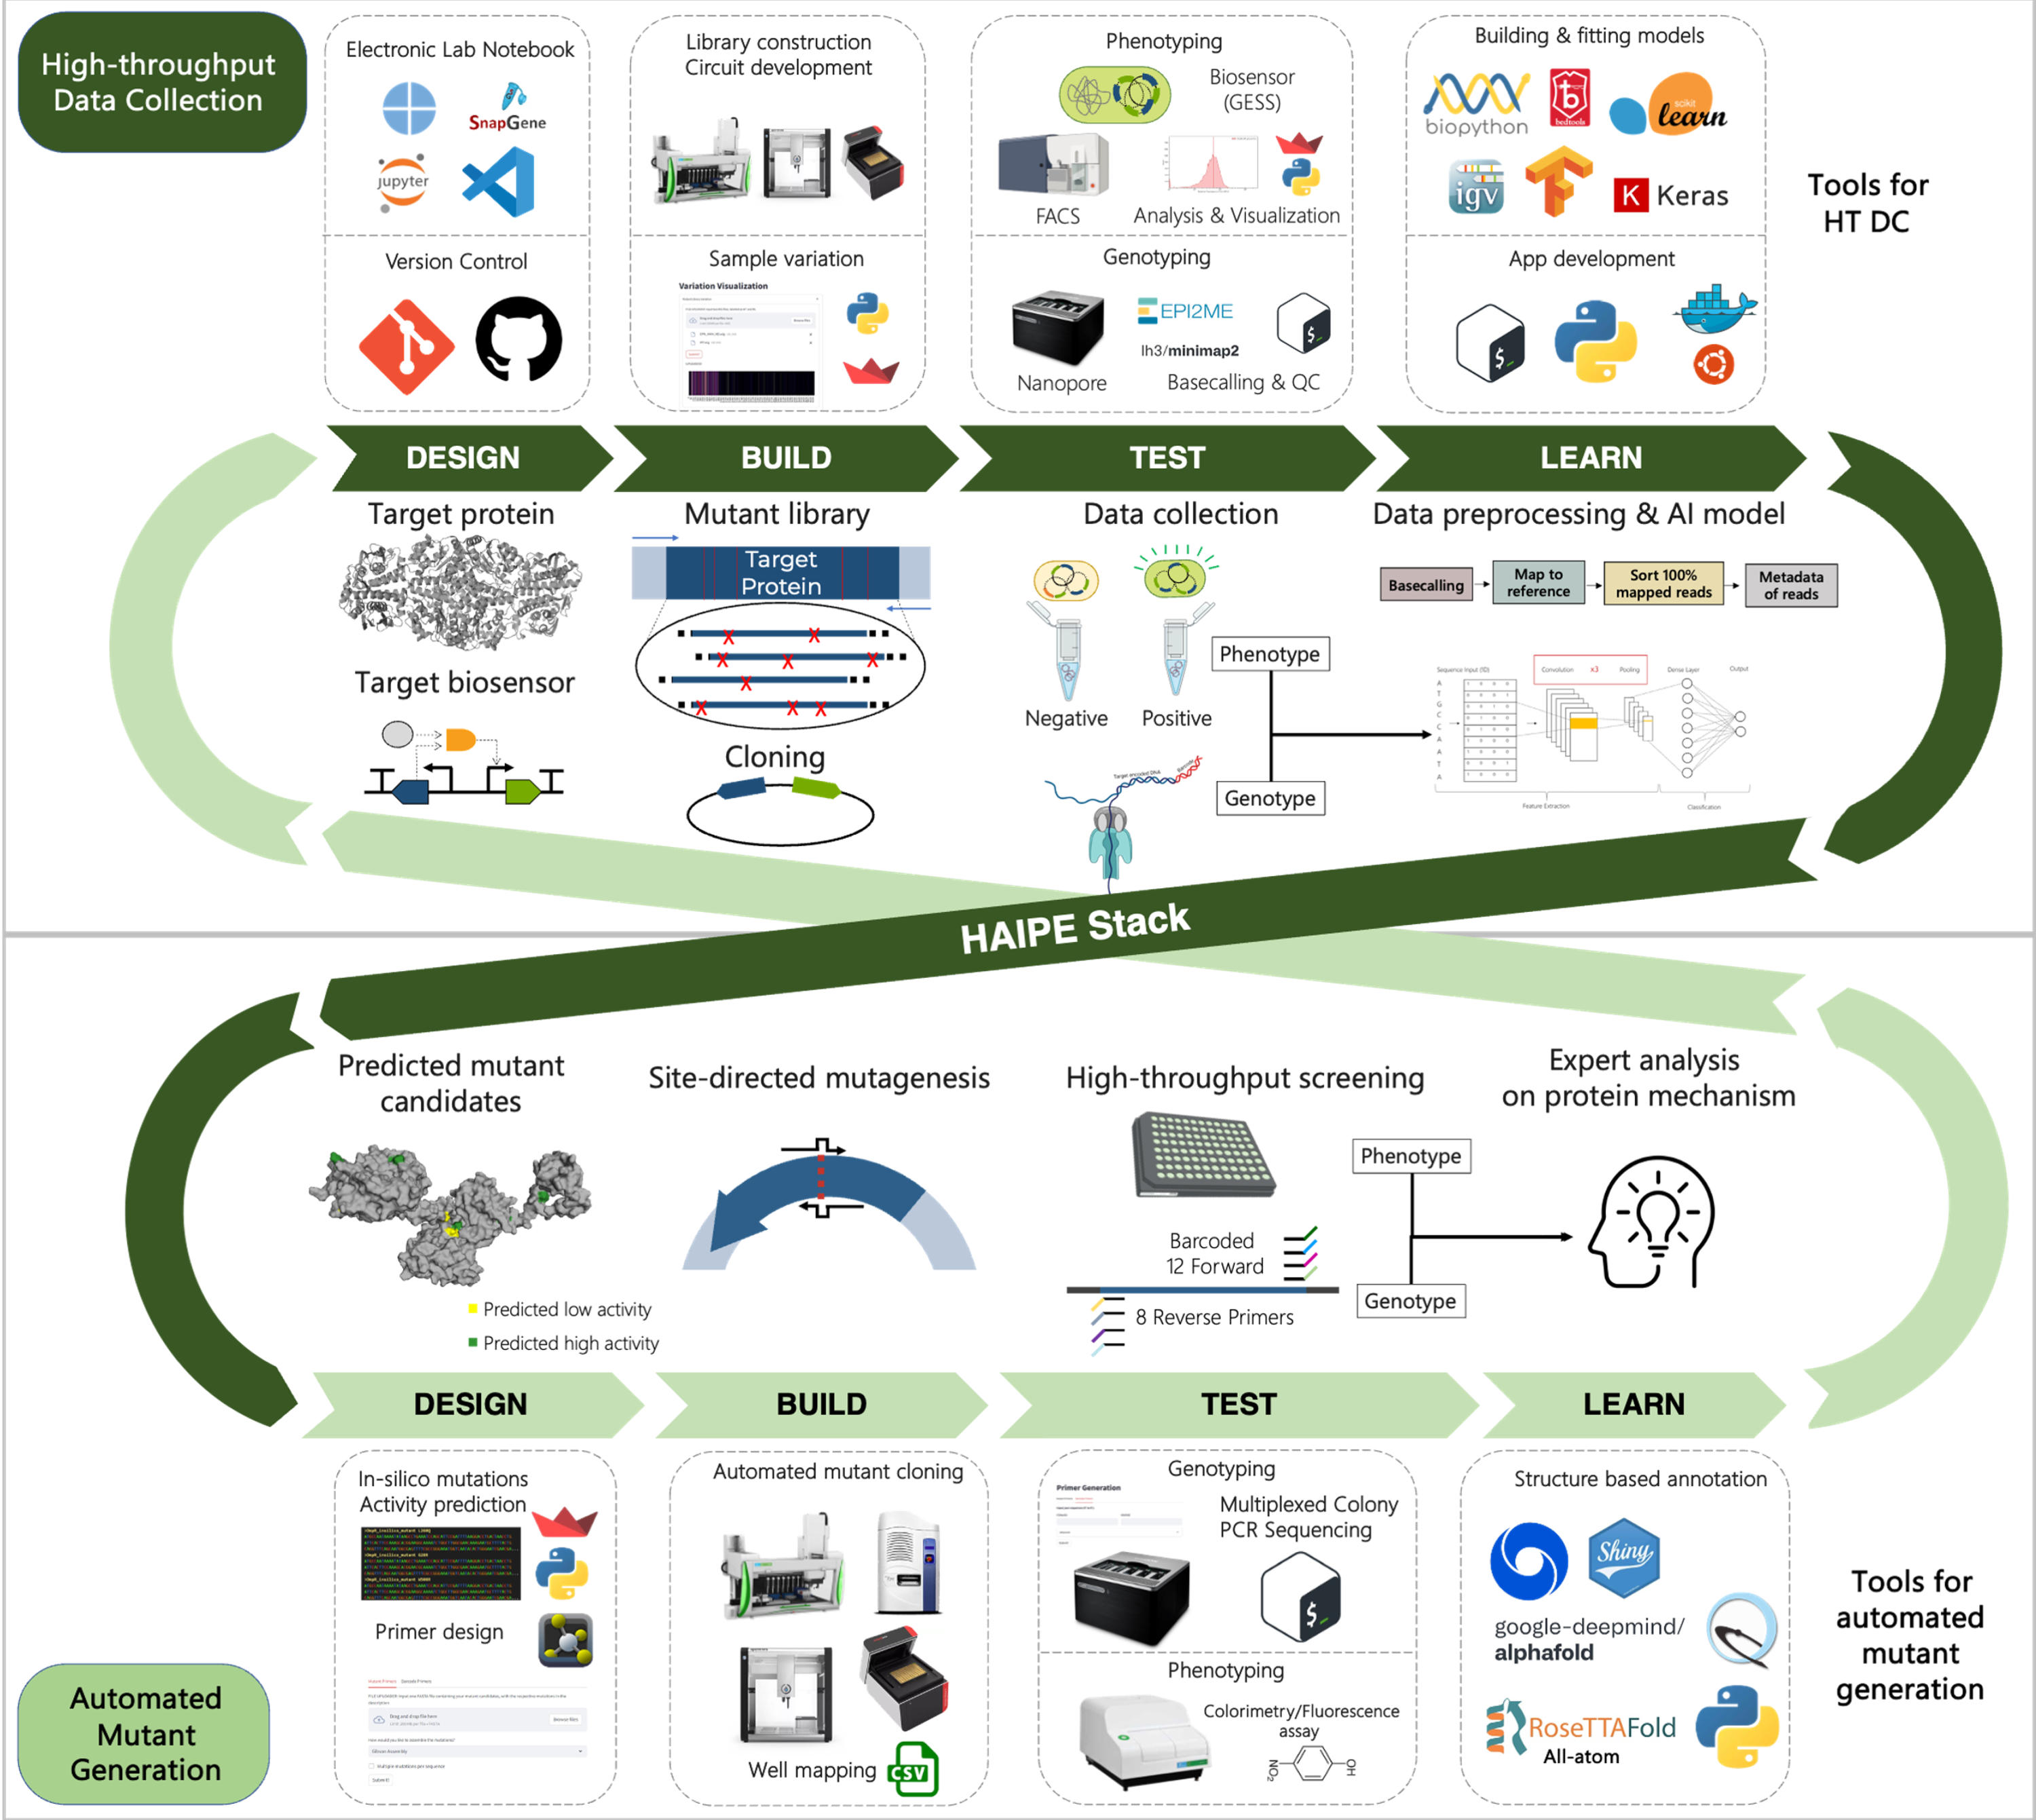
\includegraphics{chapters/images/HiAPE.png}

This thesis focuses on the development of workflows and software tools
with a focus on protein engineering.

\section{Computational Tools:}\label{computational-tools}

\subsection{Tools for Data Logging and
Collaboration:}\label{tools-for-data-logging-and-collaboration}

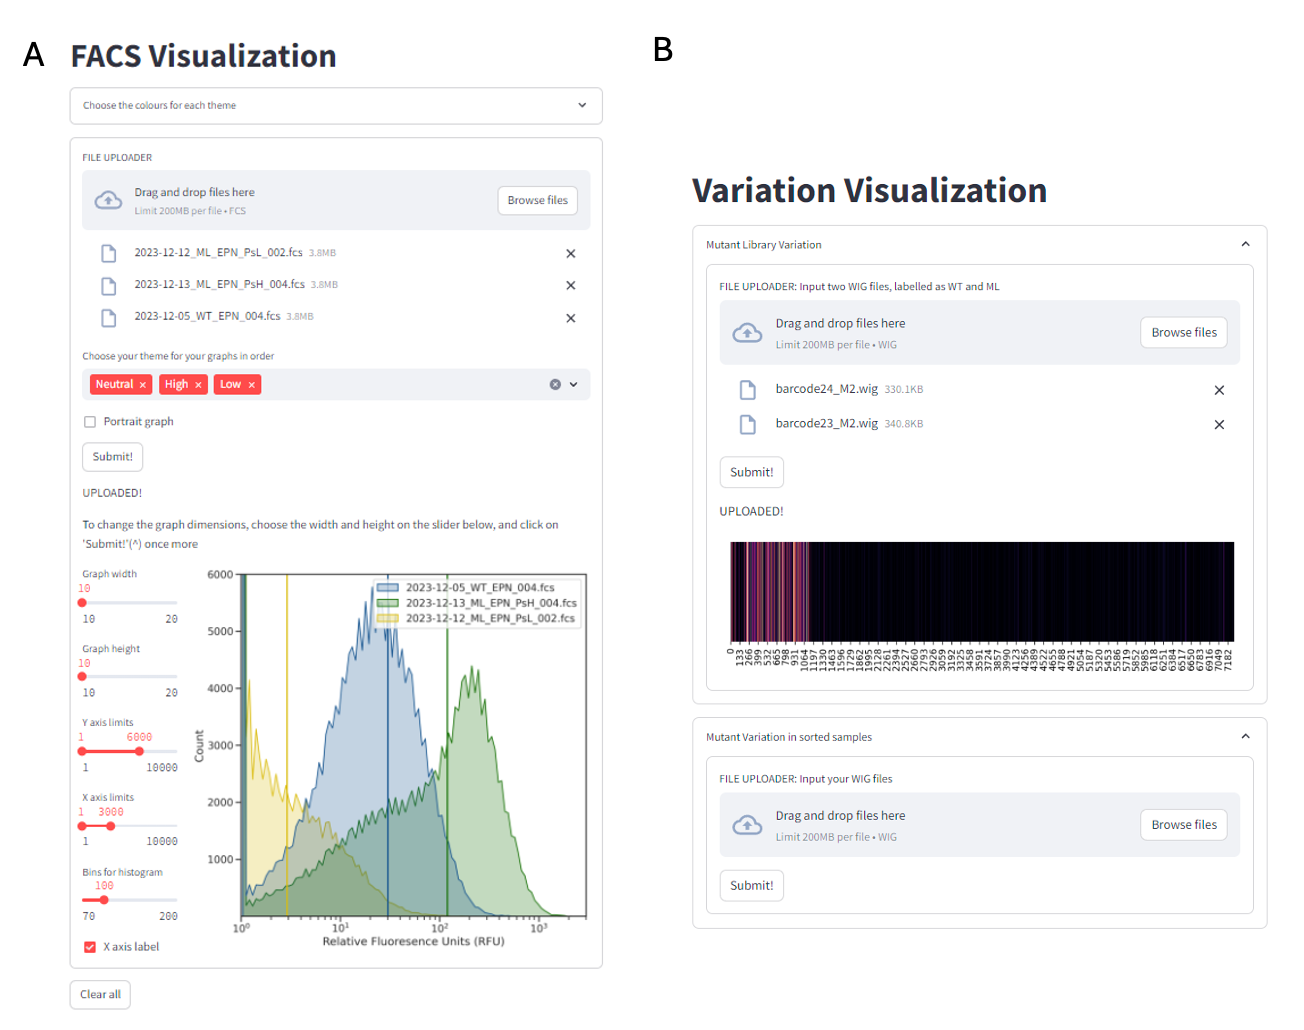
\includegraphics[width=3.66667in,height=\textheight]{chapters/images/paste-1.png}

\subsubsection{Electronic Lab
Notebooks:}\label{electronic-lab-notebooks}

Electronic Lab Notebooks (ELNs) are essential tools in modern research
environments, offering several key advantages over traditional paper
notebooks. They facilitate efficient data management by allowing
researchers to easily organize, store, and retrieve experimental data.
ELNs enhance collaboration among team members by enabling real-time
sharing and commenting on data, which fosters greater communication and
collective insights. Moreover, they improve data integrity and
reproducibility through built-in version control and automated backups,
reducing the risk of data loss or errors. ELNs also streamline
compliance with regulatory requirements by providing secure, auditable
records of experiments. Additionally, their integration with other
digital tools and platforms can enhance workflows and automate routine
tasks, ultimately increasing productivity and accelerating the research
process{[}10{]}.

While there are free options for ELN software, many vendors limit data
storage, file sizes, and the number of users, which can hinder larger
teams or projects. Portability of files can also be a concern depending
upon the ELN provider; for example if it ceases operations or raises
prices, users may only receive a PDF export of their data, complicating
transitions to other platforms. Although infrequent, security breaches,
are a potential risk that users should be aware of. Additionally, not
all electronic solutions cater to every lab's needs; for example, some
ELNs do not integrate with specific biotools like CRISPR/Cas9 genome
editing software. Furthermore, user experience can vary significantly;
many reviews point out issues with nonintuitive interfaces and the need
for extensive training, which can slow down effective implementation in
the lab {[}11{]}.

Here, we describe using Visual Studio (VS) Code along with quarto
markdown files as an ELN. VS Code is compatible with most types of
files. VS Code allows for the creation of Markdown files, which can be
used to document experiments, protocols, and results in a structured and
easily readable format. The built-in version control system (Git)
enables users to track changes over time, making it simple to maintain a
history of experiments and revisions. Open-sourced extensions allow
integration of other software such as Docker, GitHub, and Notion which
can be standardized through a free account.

Moreover, integration of Jupyter Notebooks allow for interactive data
analysis and visualization, integrating coding directly with
documentation. This can be particularly useful for analyzing data using
programming languages such as Python or R. Users can also benefit from
VS Code's robust search capabilities, making it easy to locate specific
notes or data points across multiple files. Overall, using VS Code as an
ELN combines flexibility, organization, and collaboration, making it a
compelling choice for researchers looking to streamline their
documentation processes.

\subsubsection{Version Control:}\label{version-control}

Collaboration is streamlined on GitHub, as multiple team members can
work on the same project simultaneously. Additionally, the ability to
store files in cloud-based repositories (like GitHub or GitLab) ensures
data portability and accessibility, even if the original workspace
changes. This allows users to track changes over time, providing a clear
history of modifications, which is essential for reproducibility and
accountability. Users can create branches to explore new ideas or
experiment with changes without affecting the main content. Pull
requests enable thorough discussions and reviews of proposed changes
before merging, ensuring that all contributions are vetted and enhancing
the quality of the documentation.

GitHub also supports Markdown, making it easy to format notes for
clarity and readability. With features like issue tracking, users can
manage tasks and monitor project progress efficiently. The platform's
cloud-based storage ensures that data is accessible from anywhere,
minimizing the risk of loss. Overall, using GitHub for version control
in an ELN not only improves organization and collaboration but also
enhances the integrity and transparency of the research process.

Using Docker to share workflow environments offers a powerful solution
for ensuring consistency and reproducibility in research and development
projects. Docker allows users to create containerized environments that
encapsulate all necessary dependencies, libraries, and configurations
required to run a specific application or workflow. This means that
researchers can share their entire computational environment, ensuring
that collaborators can run the same code with the same results,
regardless of their local setups.

By creating a Docker image, users can package their workflows along with
any required software, making it easy to distribute and deploy on any
system that supports Docker. This eliminates the common ``it works on my
machine'' problem, as the container will behave the same way on any
platform. Additionally, Docker supports versioning, allowing teams to
track changes in their environment over time and roll back to previous
configurations if needed. {[}12, 13{]}

Models and datasets can be uploaded on AI sharing platforms such as
Huggingface.

\subsection{Accesibility to Modelling
Tools:}\label{accesibility-to-modelling-tools}

Simulation and modeling tools play a crucial role in understanding and
optimizing biological processes, particularly in fields like systems
biology, synthetic biology, and drug development. However, many of these
advanced tools are often limited in accessibility and user-friendliness,
which can restrict their widespread adoption and effective use in
research and application.

Many of the available tools require specialized knowledge of programming
and mathematical modeling, creating a steep learning curve for
researchers who may not have a strong computational background. This can
discourage scientists from utilizing these tools, even when they could
significantly enhance their research. Additionally, some tools may lack
comprehensive documentation or user support, making it difficult for
users to troubleshoot issues or fully leverage the tool's capabilities.

Even when large models are made accessible on platforms like Google
Colab, such as ColabFold, their functionality can be limited due to
several factors. Firstly, computational resources on free or tiered
cloud platforms may be restricted, leading to longer processing times or
the inability to run particularly large or complex models that require
significant computational power. This limitation can frustrate users who
need to conduct extensive simulations or analyses. Additionally, Colab's
environment may not support all the necessary libraries or specific
versions of software that users require for their models. While Colab
offers a range of pre-installed packages, researchers may still
encounter compatibility issues, requiring extra time to set up their
environments properly. Furthermore, the reliance on internet
connectivity can also pose challenges. Interruptions or slow connections
can hinder users' ability to run or save their work, potentially
resulting in data loss or incomplete analyses {[}14{]}. Having locally
hosted databases and models downloaded allows for more accurate analysis
and predictions {[}15{]}.

To address these challenges, there is a growing need for more intuitive
simulation and modeling tools that offer user-friendly interfaces and
robust support for data integration. Enhancements such as visual
modeling environments, drag-and-drop functionalities, and real-time
feedback can make these tools more accessible to a broader audience.
Furthermore, fostering collaborations between computational scientists
and biologists can help ensure that the tools developed are tailored to
the specific needs of the research community. {[}16{]}

\subsubsection{AlphaFold/RosettaFold UI:}\label{alphafoldrosettafold-ui}

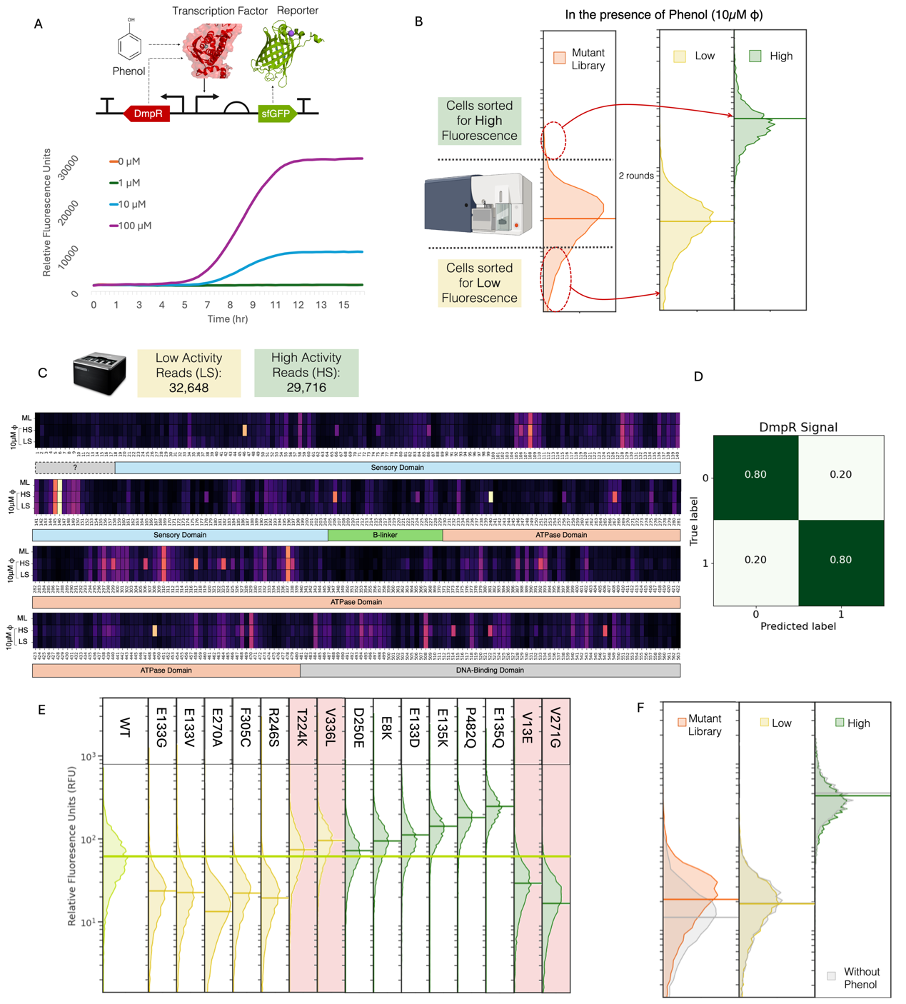
\includegraphics[width=2.65625in,height=\textheight]{chapters/images/paste-2.png}

\subsection{Visualization Tools:}\label{visualization-tools}

Biological data can be intricate and multidimensional, often involving
large datasets from experiments such as genomics, proteomics, and
metabolomics. Visualization tools help translate this data into
graphical formats, making it easier for researchers to identify
patterns, trends, and anomalies that might not be apparent in raw data.
{[}17{]}

These tools facilitate exploratory data analysis, allowing scientists to
visualize relationships and interactions among biological variables. For
instance, network diagrams can depict interactions between proteins,
while heatmaps can show gene expression levels across different
conditions, helping researchers draw meaningful conclusions and generate
hypotheses. {[}18,19, 20{]}

\subsubsection{FACS Visualization:}\label{facs-visualization}

\subsubsection{Mutant Variability
Visualizer:}\label{mutant-variability-visualizer}

\subsection{Design Tools:}\label{design-tools}

\subsubsection{Primer design:}\label{primer-design}

\subsubsection{In-silico Mutant
Generator:}\label{in-silico-mutant-generator}

\subsection{Machine Interoperability:}\label{machine-interoperability}

\subsubsection{Well Mapping:}\label{well-mapping}

\subsection{Analysis Tools:}\label{analysis-tools}

\subsubsection{Nanopore Analysis:}\label{nanopore-analysis}

\subsection{Tools for Data Storage and
Sharing:}\label{tools-for-data-storage-and-sharing}

\subsubsection{Server Management:}\label{server-management}

\bookmarksetup{startatroot}

\chapter{References}\label{references}

\begin{enumerate}
\def\labelenumi{\arabic{enumi}.}
\item
  Hodgman CE, Jewett MC (2012) Cell-free synthetic biology: thinking
  outside the cell. Metab Eng 14:261--269. https://doi.org/
  10.1016/j.ymben.2011.09.002
\item
  King RD, Whelan KE, Jones FM et al (2004) Functional genomic
  hypothesis generation and experimentation by a robot scientist. Nature
  427:247--252. https://doi.org/10.1038/nature02236
\item
  King RD, Rowland J, Oliver SG et al (2009) The automation of science.
  Science 324:85--89. https://doi.org/10.1126/science. 1165620
\item
  Köpke M, Simpson SD (2020) Pollution to products: recycling of ``above
  ground'' carbon by gas fermentation. Curr Opin Biotechnol 65:180--189.
  https://doi.org/10.1016/j.copbio.2020.02.017
\item
  Vögeli B, Schulz L, Garg S et al (2022) Cell-free prototyping ena-
  bles implementation of optimized reverse β-oxidation pathways in
  heterotrophic and autotrophic bacteria. Nat Commun 13:3058.
  https://doi.org/10.1038/s41467-022-30571-6
\item
  Kim KJ, Lee SJ, Kim DM (2023) The use of cell-free protein synthesis
  to push the boundaries of synthetic biology. Biotechnol Bioprocess
  Eng. https://doi.org/10.1007/s12257-022-0279-2
\item
  Kelly J (2022) Grow with ginkgo. Ginkgo Bioworks. https://s28.
  q4cdn.com/823357996/files/doc\_presentations/2022/01/2022.01.
  12-Ginkgo-DNA-JPM-2022.pdf.
\item
  \url{https://www.cowen.com/transactions/amyris-inc-6-4-2020/}
\item
  Sogi GM (2023) Research waste. Contemp Clin Dent 14:179.
\item
  Kwok R (2018) How to pick an electronic laboratory notebook. Nature
  560:269--270. https:// doi. org/ 10. 1038/ d41586-018-05895-3
\item
  \url{https://www.idtdna.com/pages/community/blog/post/thinking-about-making-the-switch-to-an-electronic-lab-notebook-here-are-some-pros-and-cons}
\item
  David Eyers, Sarah Stevens, Andy Turner and Jeremy Cohen, Containers
  for reproducible research.
  \url{https://github.com/ImperialCollegeLondon/2020-07-13-Containers-Online/blob/gh-pages/CITATION}
\item
  Leahy, Darragh, and Christina Thorpe. ``Zero trust container
  architecture (ztca): A framework for applying zero trust principals to
  docker containers.'' \emph{International Conference on Cyber Warfare
  and Security}. Vol. 17. No.~1. 2022.
\item
  Mirdita, M., Schütze, K., Moriwaki, Y., Heo, L., Ovchinnikov, S. and
  Steinegger, M., 2022. ColabFold: making protein folding accessible to
  all. \emph{Nature methods}, \emph{19}(6), pp.679-682.
\item
  Jumper, J., Evans, R., Pritzel, A., Green, T., Figurnov, M.,
  Ronneberger, O., Tunyasuvunakool, K., Bates, R., Žídek, A., Potapenko,
  A. and Bridgland, A., 2021. Highly accurate protein structure
  prediction with AlphaFold. \emph{nature}, \emph{596}(7873),
  pp.583-589.
\item
  Eblen-Zayas, M., 2015. Comparing electronic and traditional Lab
  Notebooks in the advanced lab. In \emph{Conference on Laboratory
  Instruction: Beyond the First Year of College, College Park, MD.
  Retrieved from https://www. compadre.
  org/Repository/document/ServeFile. cfm}.
\item
  Wong, B., 2012. Visualizing biological data. \emph{Nat Methods},
  \emph{9}(12), pp.1131-1131.
\item
  \url{https://github.com/keller-mark/awesome-biological-visualizations}
\item
  Verschaffelt, P., Collier, J., Botzki, A., Martens, L., Dawyndt, P.
  and Mesuere, B., 2022. Unipept Visualizations: an interactive
  visualization library for biological data. \emph{Bioinformatics},
  \emph{38}(2), pp.562-563.
\item
  Kerren, A., Kucher, K., Li, Y.F. and Schreiber, F., 2017. BioVis
  Explorer: A visual guide for biological data visualization techniques.
  \emph{PLoS One}, \emph{12}(11), p.e0187341.
\end{enumerate}

\bookmarksetup{startatroot}

\chapter{Data Collection for AI-based Protein
Engineering}\label{data-collection-for-ai-based-protein-engineering}

\section{Introduction}\label{introduction-2}

\begin{itemize}
\item
  Problems with Protein Engineering
\item
  AI solutions
\item
  Problems with AI based Engineering
\end{itemize}

\section{Design}\label{design}

\begin{itemize}
\item
  Biosensor
\item
  ELN
\item
  Server Conformity
\end{itemize}

\section{Build}\label{build}

\begin{itemize}
\item
  Gibson Assembly
\item
  Mutant Library
\end{itemize}

\section{Test}\label{test}

\begin{itemize}
\item
  FACS
\item
  Nanopore Sequencing
\item
  FACS Visualization
\end{itemize}

\section{Learn}\label{learn}

\begin{itemize}
\item
  Data Processing
\item
  AI
\item
  Binary Relevance vs Classifier vs Multiclass Classifications
\end{itemize}

\section{Evaluations}\label{evaluations}

\begin{itemize}
\item
  DmpR
\item
  MPH
\end{itemize}

\section{Future Considerations}\label{future-considerations}

\bookmarksetup{startatroot}

\chapter{Biofoundry based production of mutants and long DNA
sequences}\label{biofoundry-based-production-of-mutants-and-long-dna-sequences}

\section{Introduction}\label{introduction-3}

\section{Design}\label{design-1}

\begin{itemize}
\item
  In-silico Modelling:

  \begin{itemize}
  \item
    Random
  \item
    Generative AI
  \end{itemize}
\item
  Primer Design
\item
  Biofoundry equipment mapping
\end{itemize}

\section{Build}\label{build-1}

\begin{itemize}
\tightlist
\item
  SDM
\end{itemize}

\newpage

\section{Test: High-throughput mutant
screening}\label{test-high-throughput-mutant-screening}

\subsection{Multiplexed barcode PCR
sequencing}\label{multiplexed-barcode-pcr-sequencing}

\subsection{Nanopore analysis}\label{nanopore-analysis-1}

The output of the Nanopore sequencing is the pooled result of the above
PCR products, which comprises of different samples with different
samples. It is important to demultiplex the samples to differentiate the
sequences appropriately. Follow the steps to run

\subsection{Phenotyping}\label{phenotyping}

\newpage

\section{Learn}\label{learn-1}

\begin{itemize}
\tightlist
\item
  Structure Predictions and Simulations
\end{itemize}

\bookmarksetup{startatroot}

\chapter{Dsembler - DNA Assembly Designer: A tool for Facilitating
Assembly of Long
DNA}\label{dsembler---dna-assembly-designer-a-tool-for-facilitating-assembly-of-long-dna}

\section{Introduction}\label{introduction-4}

\begin{itemize}
\item
  Literature Review of Traditional Synthetic Biology design rules
\item
  Constructing plasmids and genomes
\item
  Limited tools/ Not better than manually working though them- Labour
  intensive
\item
  Synthesizing Large fragments is challenging
\end{itemize}

\section{Consideration for designing
oligomers}\label{consideration-for-designing-oligomers}

\begin{itemize}
\item
  Number of overlaps
\item
  No repeats
\item
  GC\%
\item
  No A at 3' end
\end{itemize}

\section{Psuedocode}\label{psuedocode}

\section{User Interface}\label{user-interface}

\begin{itemize}
\item
  Python- Flask
\item
  R- Shiny
\end{itemize}

\section{Experimental Evaluation}\label{experimental-evaluation}

\subsection{Materials and Methods}\label{materials-and-methods}

\begin{itemize}
\tightlist
\item
  Role of Biofoundry
\end{itemize}

\subsection{Results}\label{results}

\section{Discussion}\label{discussion}

\begin{itemize}
\tightlist
\item
  Integrating with the Biofoundry and sample tracking to mass produce
  samples
\end{itemize}

\bookmarksetup{startatroot}

\chapter*{Conclusion}\label{conclusion}
\addcontentsline{toc}{chapter}{Conclusion}

\markboth{Conclusion}{Conclusion}

\bookmarksetup{startatroot}

\chapter*{References}\label{references-1}
\addcontentsline{toc}{chapter}{References}

\markboth{References}{References}

\phantomsection\label{refs}
\begin{CSLReferences}{0}{1}
\end{CSLReferences}

\bookmarksetup{startatroot}

\chapter*{Appendix}\label{appendix}
\addcontentsline{toc}{chapter}{Appendix}

\markboth{Appendix}{Appendix}

\begin{figure}[H]

{\centering 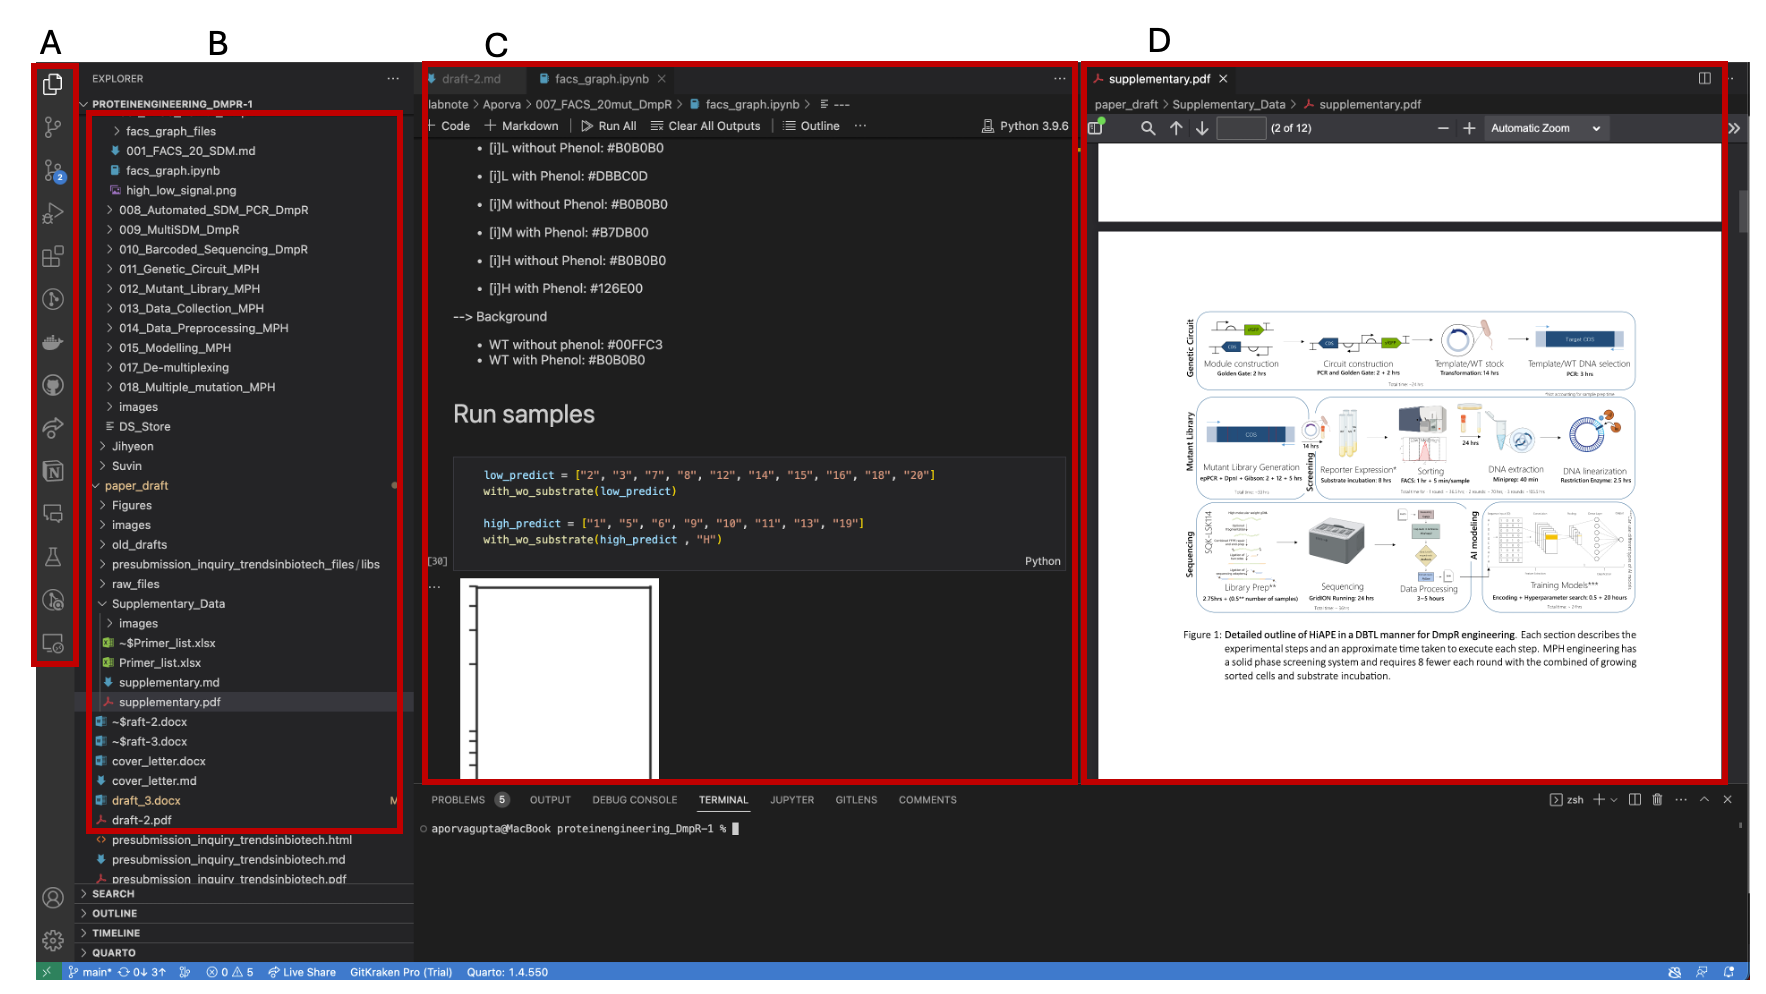
\includegraphics{chapters/images/VS_code.png}

}

\caption{A: Activity Bar showcasing the extensions installed locally. B:
Primary Side Bar that displays the layout of files and Source code
changes. C: Main window to edit markdown and jupyter notebook files. D:
A Preview panel to view PDF and HTML files.}

\end{figure}%


\backmatter

\end{document}
